\section{SmartLightingKit}

SmartLightingKit is a system expected to manage the lights of a potentially big building composed of many rooms (e.g., an office space).
Each room of the building, may have one or more lights.
The system shall allow the lights to be controlled (either locally or remotely) by authorized users. 
Local control is achieved through terminals installed in the rooms (one terminal per room). 
Remote control is realized through a smartphone application, or through a central terminal installed in the control room of the building.
While controlling the lights of a room, the user can execute one or more of the following actions: turn a light on/off at the current time, at a specified time, or when certain events happen (e.g., a person enters the building or a specific room). 
Moreover, users can create routines, that is, scripts containing a set of actions.
SmartLightingKit manages remote control by adopting a fine-grained authorization mechanism.
This means there are multiple levels of permissions that may even change dynamically.
System administrators can control the lights of every room, install new lights, and remove existing ones. 
This diagram describes the portion of the SmartLightingKit system supporting lights turning on/off and lights status checking.
\begin{figure}[H]
    \centering
    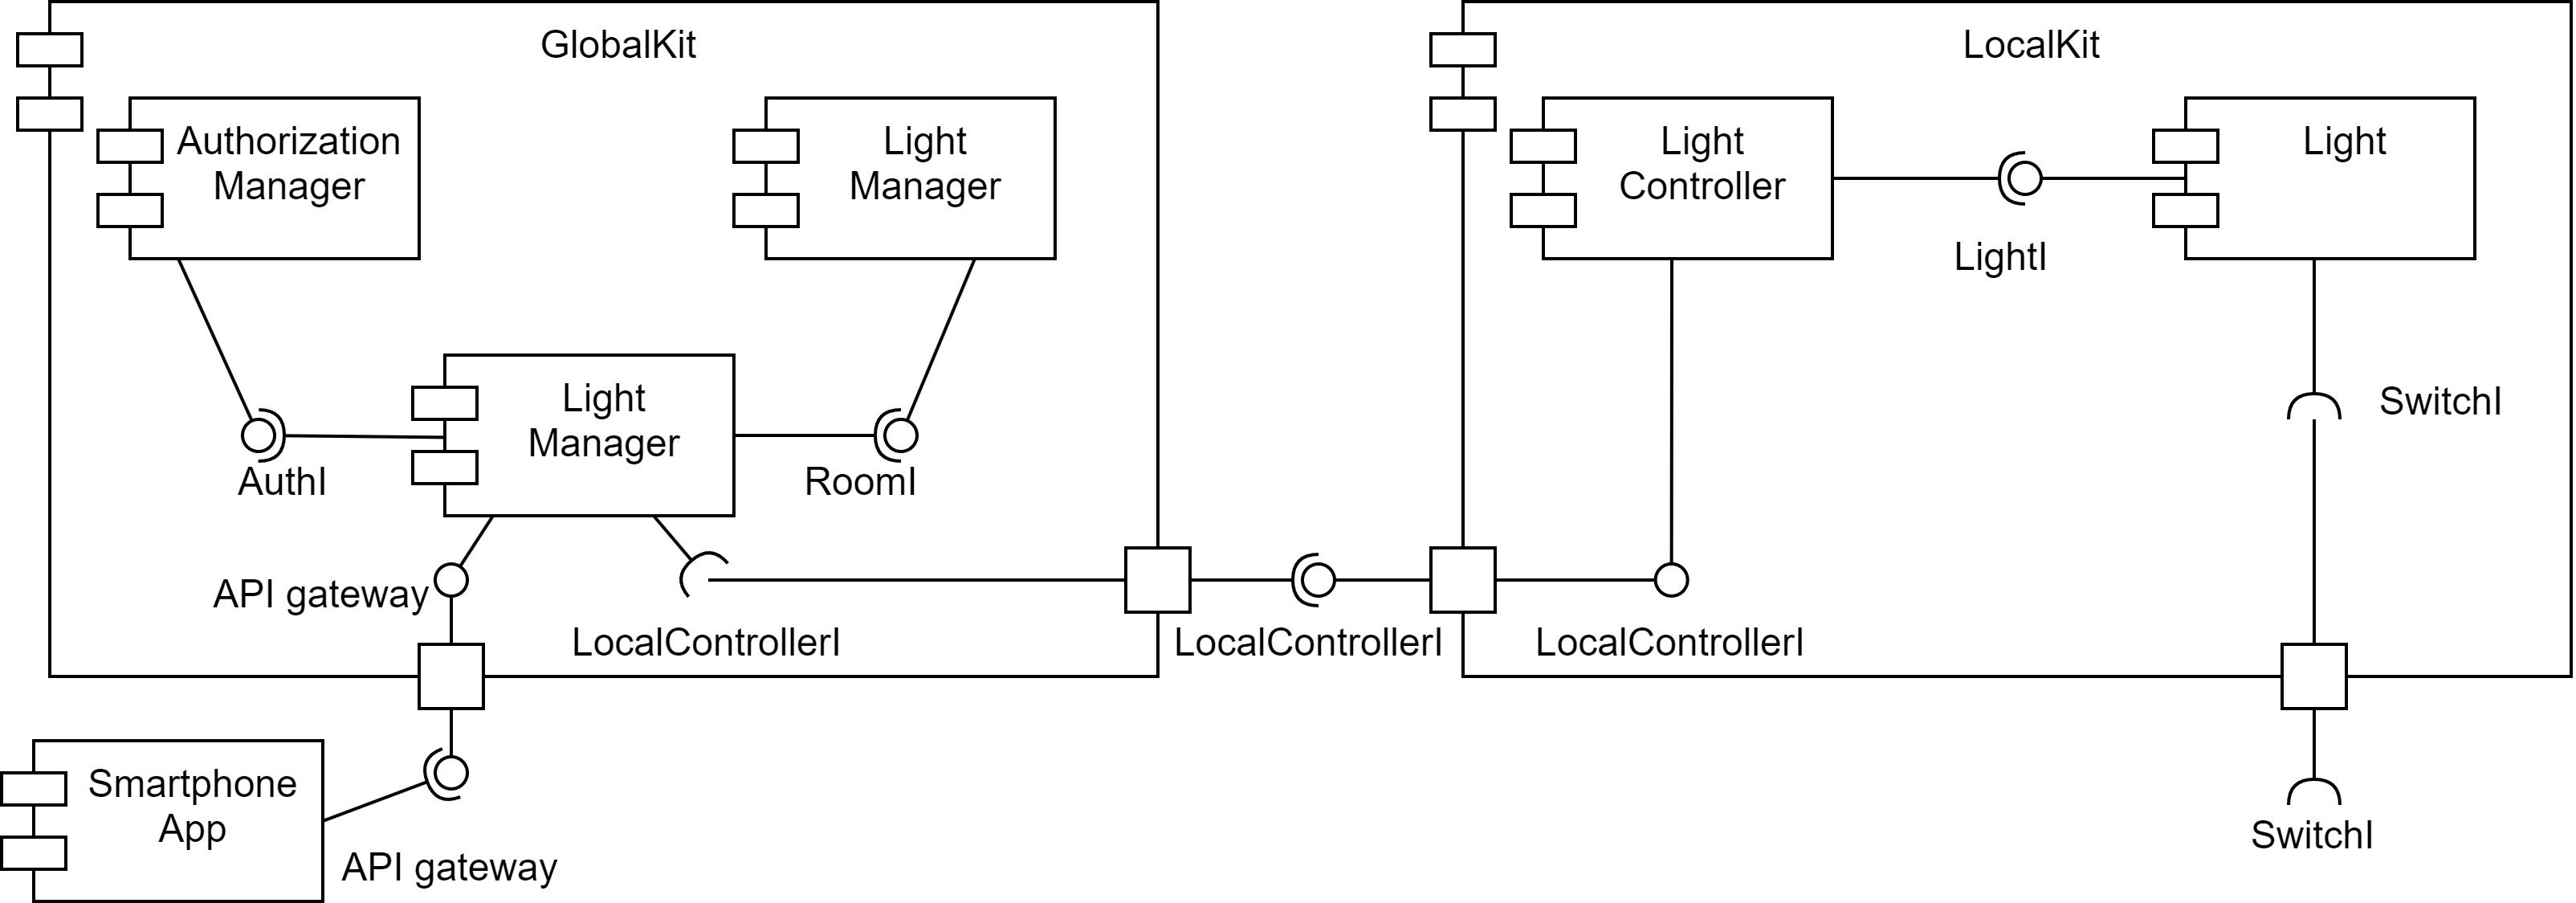
\includegraphics[width=0.9\linewidth]{images/uml1.png}
\end{figure}
The diagram is complemented by the following description.
\texttt{GlobalKit} is the component installed in the central terminal. 
It can be contacted through the \texttt{APIGateway} interface by the \texttt{SmartphoneApp} component representing the application used for remote control. 
\texttt{GlobalKit} includes:
\begin{itemize}
    \item \texttt{RoomMapping}, which keeps track, in a persistent way, of lights' locations within the building's rooms. 
    \item \texttt{AuthorizationManager}, which keeps track, in a persistent way, of the authorizations associated with each user (for simplicity, we assume that users exploiting the operations offered by the \texttt{APIGateway} are already authenticated through an external system and include in their operation calls a proper token that identifies them univocally);
    \item \texttt{LightManager}, which coordinates the interaction with all \texttt{LocalKit} components.
\end{itemize}
Each \texttt{LocalKit} component runs on top of a local terminal. 
Also, each \texttt{LocalKit} exposes the \texttt{LocalControllerI} interface that is implemented by its internal component \texttt{LightController}, which controls the lights in the room. 
Each light is represented in the system by a Light component which interacts with the external system operating the light through the \texttt{switchCommand} operation offered by the latter.
\begin{enumerate}
    \item Analyze the operations offered by the components shown in the diagram and identify proper input and output parameters for each of them.
    \item Write a UML Sequence Diagram illustrating the interaction between the software components when a regular user wants to use the smartphone application to check whether he/she left some lights on (among the lights he/she can control).
    \item Assume that, at a certain point, the following new requirement is defined:
        “The smartphone application should allow users to activate and deactivate the receival of real-time updates about the state (on/off) of all the lights they can control.”
        Define a high-level UML Sequence Diagram to describe how the current architecture could accommodate this requirement.
        Highlight the main disadvantage emerging from the sequence diagram.
\end{enumerate}

\paragraph*{Solution}
\begin{enumerate}
    \item The \texttt{APIGateway} has the following methods: 
        \begin{itemize} 
            \item \texttt{getLights}. 
                The input of this method is the \texttt{userID}.
                The output of this method is \texttt{list[lightID]}.
            \item \texttt{getState}.
                The input of this method is the \texttt{userID}.
                The output of this method is \texttt{list[(lightID, state)]}.
            \item \texttt{setState}.
                The inputs of this method are the \texttt{userID}, \texttt{lightID}, and \texttt{state}.
                The output of this method is \texttt{none}.
        \end{itemize}
        The \texttt{AuthI} has the following method: 
        \begin{itemize} 
            \item \texttt{getAuthorizations}. 
                The input of this method is the \texttt{userID}.
                The output of this method is \texttt{list[(roomID, localKitID)]}.
        \end{itemize}
        The \texttt{RoomI} has the following method: 
        \begin{itemize} 
            \item \texttt{findLight}. 
                The input of this method is the \texttt{roomID}.
                The output of this method is \texttt{list[lightID]}.
        \end{itemize}
        The \texttt{LocalControllerI} has the following methods: 
        \begin{itemize} 
            \item \texttt{switch}. 
                The input of this method is the \texttt{lightID}.
                The output of this method is \texttt{none}.
            \item \texttt{getState}. 
                The input of this method is the \texttt{lightID}.
                The output of this method is \texttt{state}.
        \end{itemize}
        The \texttt{LightI} has the following methods: 
        \begin{itemize} 
            \item \texttt{isOn}. 
                The input of this method is the \texttt{none}.
                The output of this method is \texttt{true} or \texttt{false}.
            \item \texttt{switch}. 
                The input of this method is the \texttt{none}.
                The output of this method is \texttt{none}.
        \end{itemize}
        The \texttt{SwitchI} has the following methods: 
        \begin{itemize} 
            \item \texttt{switchCommand}. 
                The input of this method is the \texttt{none}.
                The output of this method is \texttt{none}.
        \end{itemize}
        Note that the state can be \texttt{on} or \texttt{off}. 
        Additionally, all the operations of \texttt{APIGateway}, \texttt{AuthI}, \texttt{RoomI}, \texttt{LocalKitI} receive as input also the authentication token. 
    \item The requested UML Sequence Diagram is depicted below: 
        \begin{figure}[H]
            \centering
            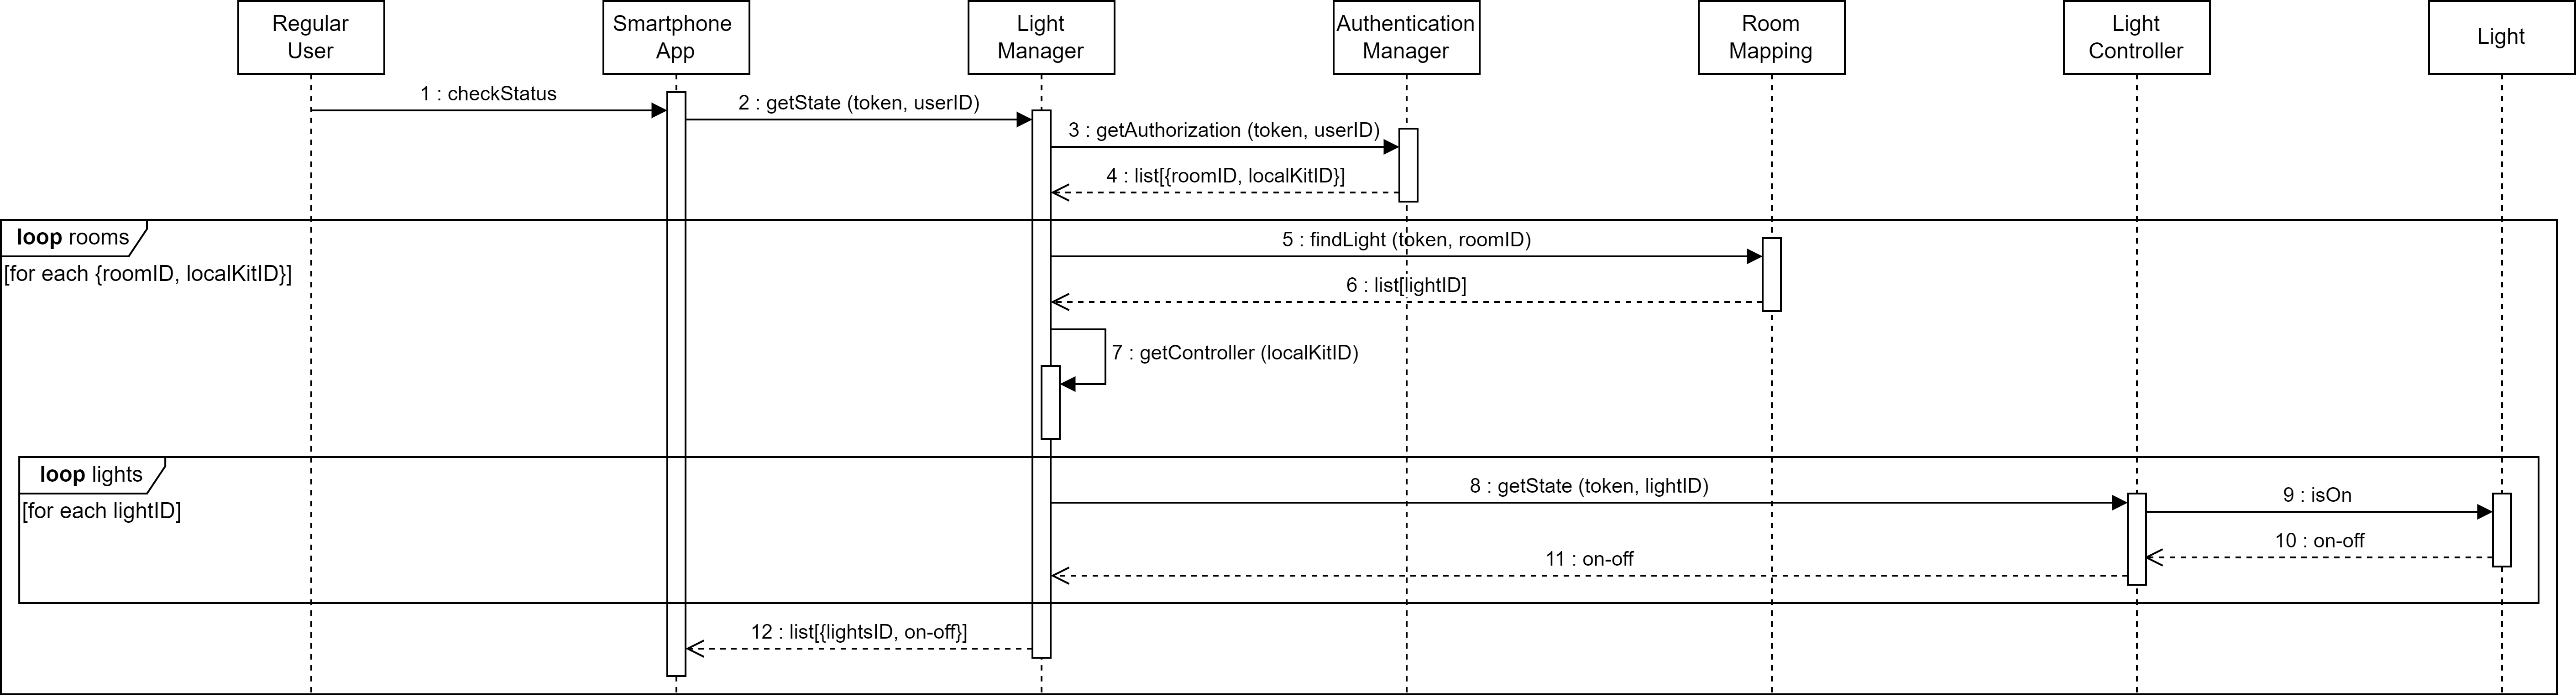
\includegraphics[width=0.9\linewidth]{images/sd.png}
        \end{figure}
    \item The requested UML Sequence Diagram is depicted below: 
        \begin{figure}[H]
            \centering
            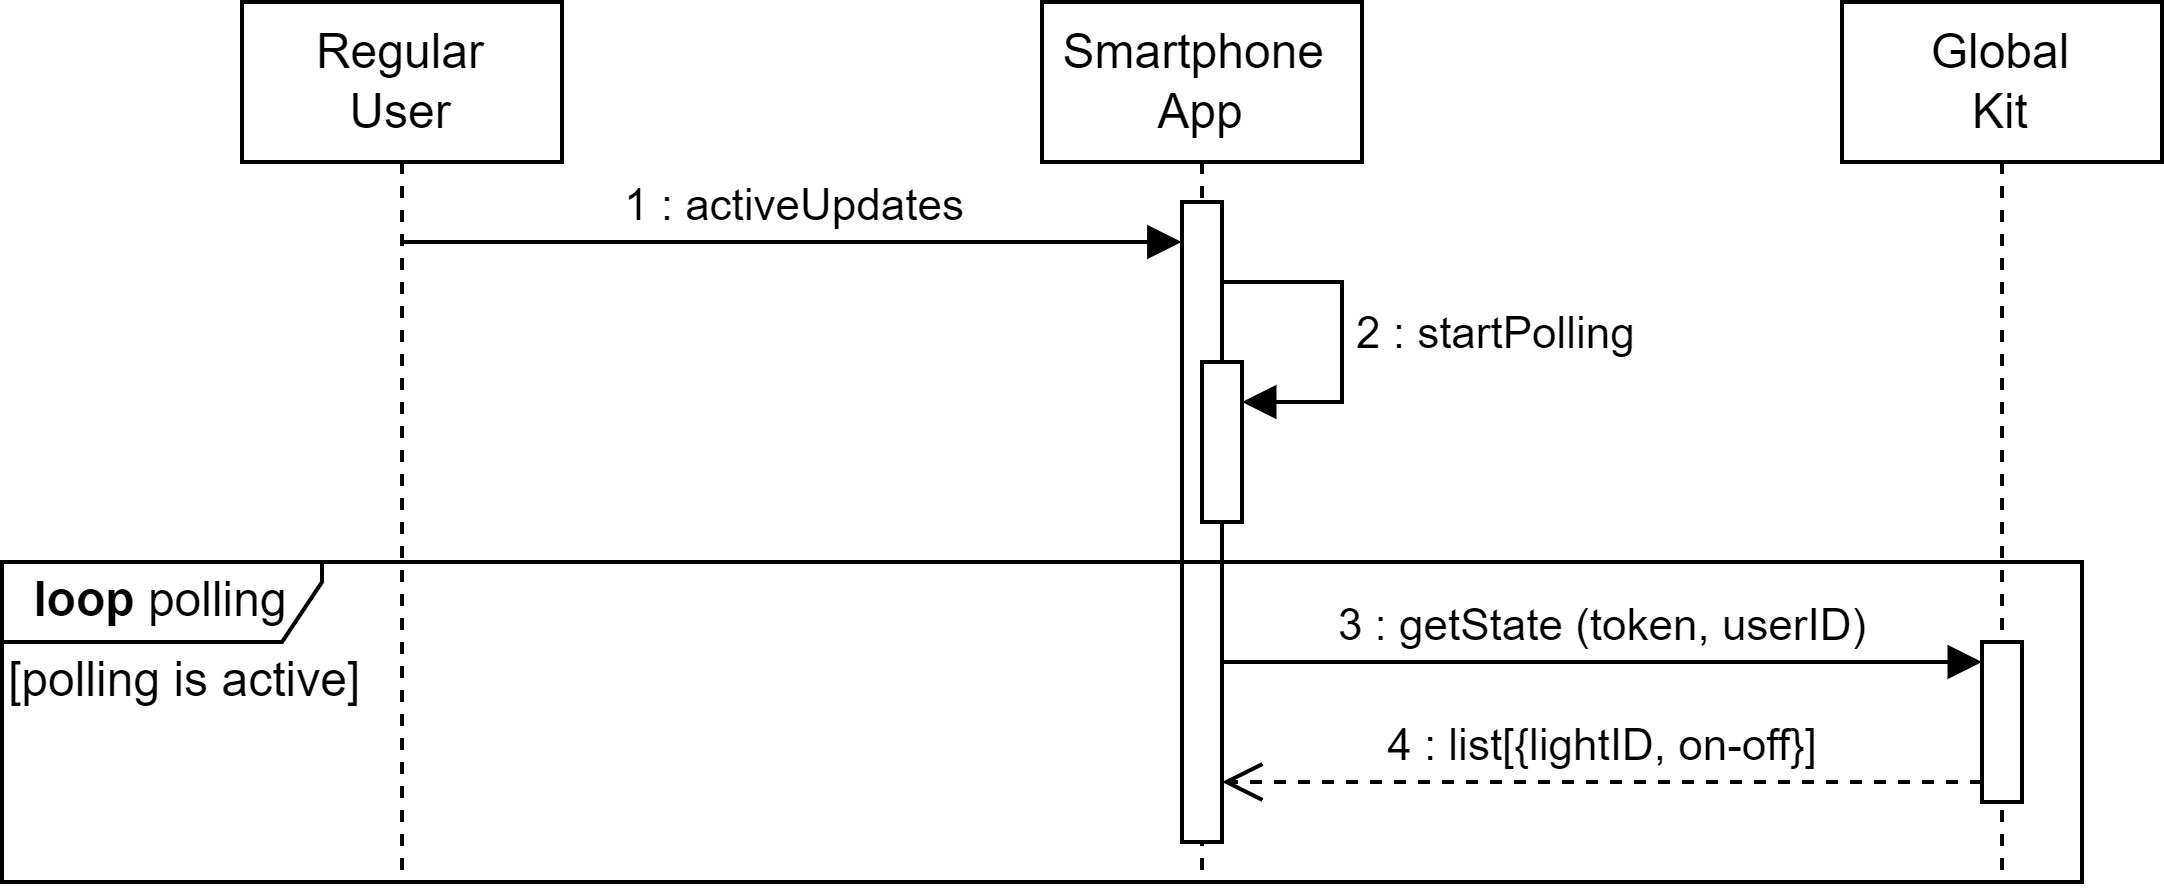
\includegraphics[width=0.8\linewidth]{images/sd1.png}
        \end{figure}
        The problems of this new feature are: 
        \begin{itemize}
            \item The current architecture does not support updates in push mode.
            \item The \textit{SmartphoneApp} carries out a continuous polling process to retrieve the status of all the lights even in case it does not change.
            \item This propagates also internally to \textit{GlobalKit} and the involve \textit{LocalKits}, thus resulting in a potentially significant communication overhead.
        \end{itemize}
\end{enumerate}